% 来源：OEBPS/Text/Section0001_split_007.xhtml#sigil_toc_id_55

\BookChapter{42}
\section[第42章\q 查尔斯·施瓦布：跟查克谈谈，他是普通人的经纪人]{第42章\\ 查尔斯·施瓦布：跟查克谈谈，他是普通人的经纪人}

\begin{figure}[htbp]
\centering
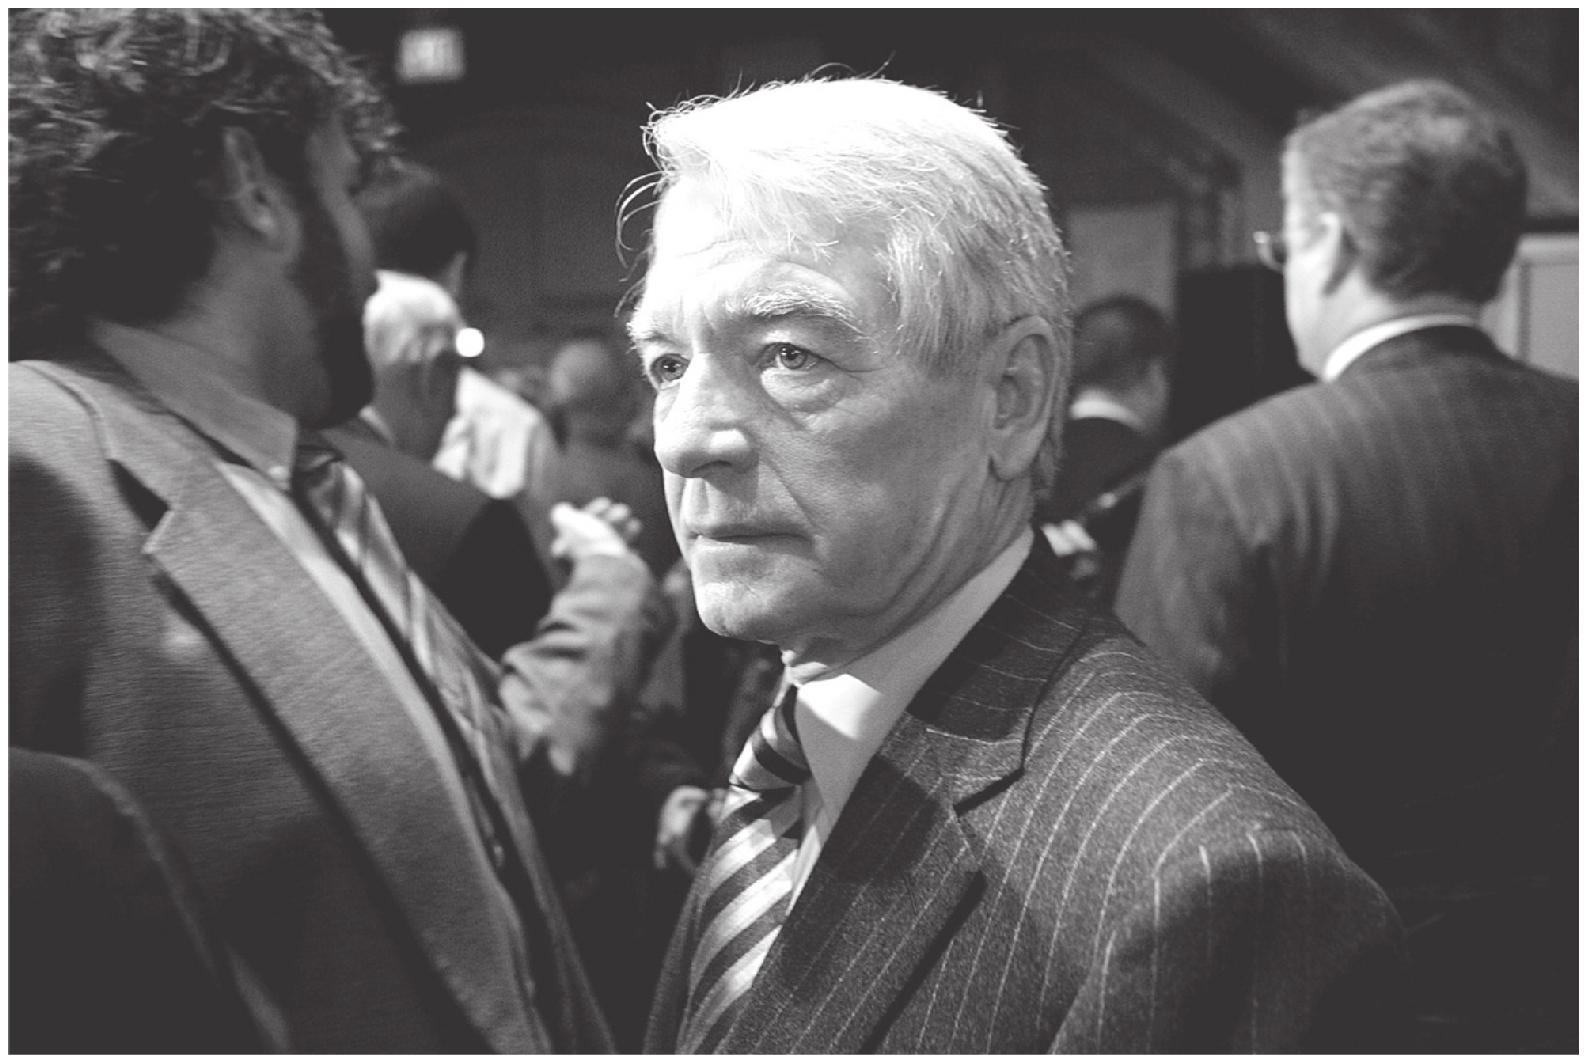
\includegraphics[width=0.56\linewidth,keepaspectratio]{image/查尔斯·施瓦布肖像.jpg}
\caption*{查尔斯·施瓦布}
\end{figure}

嘉信理财公司创始人兼董事会主席

你肯定看过这个广告：一个很帅的白发老者，两眼炯炯有神，直视着你，敦促你“要拥有自己的明天”。也许你还记得另一则广告：有些卡通人物，在问一些关于投资的问题，然后，有个气球弹出来，鼓励他们去“跟查尔斯谈谈”。这种亲身参与和坦诚交流的风格，让查尔斯·施瓦布在过去40年一直站在证券折扣经纪行业的顶峰，把嘉信理财打造成金融企业帝国，管理高达2.38万亿美元客户资产、930万个经纪账户、140万名公司退休金计划参与人、95.6万个银行账号，还有一个用于服务7000个注册投资顾问的网络。

嘉信理财公司出现之前，如果你要想买些股票，必须通过一个传统券商的卡特尔联盟，或者找一家券商，每一笔交易收的佣金都高得离谱。但是到了1975年，美国证券监督管理委员会强迫这个行业解除管制，放开佣金，查尔斯·施瓦布创办了第一个折扣经纪公司，率先探索性地用一种全新的方式来做证券经纪业务，为客户提供比同行更低的佣金折扣优惠，结果从核心上动摇了整个华尔街。查尔斯·施瓦布领导掀起一场投资者革命，突然之间，个人可以完全自主地参与市场交易，根本不需要成本很高的经纪人。那些像俱乐部一样相当排外的传统券商，比如美林证券，提高了交易手续费，而查尔斯·施瓦布大幅削减手续费，甚至完全免除手续费，提供一系列免除各种不必要手续费的服务，把客户的利益放在第一位，建立了一种新型证券经纪行业经营模式。后来查尔斯·施瓦布又带头进军电子交易领域，带头创新性地教育投资者，提高投资者的自主权，让他们能够独立地做出合理的投资决策。

2014年，查尔斯·施瓦布已经76岁了，他待人接物非常谦卑，也非常正直。“大家看起来对我们非常信任。”他对我说，“我们对待每个人，也要让人有这种感觉，我们值得他们信任，我们要用小心谨慎的方式照看好他们的资产。”

查尔斯·施瓦布为人非常谦虚稳重，做事又很有信心，这可能是多年生活经历磨炼出来的。他这辈子克服了一系列的困难挑战，一开始是跟读写障碍做斗争，就是很难学会阅读和拼写。其实很多非常成功的企业领导人从小都有读写障碍，人数多得惊人，其中包括维珍集团创始人理查德·布兰森、思科系统公司的约翰·钱伯斯等。尽管在阅读上有困难，查尔斯·施瓦布还是成功地考上斯坦福大学，也成功地毕业了，后来又读了斯坦福商学院的工商管理硕士。1963年，施瓦布进军金融行业，一开始是搞了一份投资时事通讯。施瓦布这个人不装，他轻松自然地接受了自己的身份地位——一个证券行业的外行。回到老家加利福尼亚州，他打起自己的大旗。1973年，在旧金山创立了自己的证券经纪公司，就是今天的嘉信理财公司。从此之后，嘉信理财公司风风雨雨40年，历经一轮又一轮狂暴的牛市和熊市，特别是1987年、2001年、2008年的股市大崩盘淘汰掉了那些规模较小的证券公司，嘉信理财公司却在崩盘后迅速反弹，尽管有很多同行公司抄袭嘉信理财公司的经营模式，夺走了嘉信理财公司的不少市场份额，但是嘉信理财公司总是能找到办法，不断创新，在每种市场环境下都能继续成长。

2008年施瓦布不再担任嘉信理财公司的首席执行官，但他继续担任公司的董事会主席，也仍然是公司最大的单一股东，继续活跃在公司的舞台上。按照《福布斯》400富豪排行榜的统计，查尔斯·施瓦布的个人财富有64亿美元。在他妻子和女儿嘉莉·施瓦布·波梅兰兹的协助下，他非常深入地参与家庭的私人基金会运作，支持由企业家组成的机构的慈善工作，包括教育、预防贫穷、健康卫生、公共服务。施瓦布还是旧金山现代艺术博物馆的馆长。

我一直想采访施瓦布，虽然我们两个人每天的日程表都排得满满的，但是最终我们还是想方设法地在他位于旧金山的办公室见面了，那个时候本书马上就要出版了。我们俩聊了很久，下面是一些内容节选：

\begin{BookQuote}
\textbf{罗宾斯：}每个人都知道查尔斯·施瓦布的大名，他们知道的是嘉信理财公司（公司英文名字与创始人同名——Charles Schwab），但是大多数人并不真正地了解查尔斯·施瓦布你这个公司创始人。我想请你给我们讲讲你个人的故事，讲讲你印象最深的故事，可以吗？我听说，你很小就对投资开始感兴趣了，那时你才13岁，是吗？
\end{BookQuote}

\begin{BookQuote}
\textbf{施瓦布：}对。我是在13岁开始对投资产生兴趣的，那是1950年，“二战”结束不久，整个世界还不是那么富裕。我的父亲在加利福尼亚州萨克拉门托的一个小镇上当律师，我们家肯定不是非常富有的。我想，要是我有更多的钱，我们家的生活就能过得更好一些，于是我就经常琢磨怎么样赚钱。我跟父亲谈了我想赚更多钱的理想，他鼓励我读一些美国名人传记。这些人能发大财，看来都是因为有些投资做得好。于是我就对自己说：“这就是我要干的事！”
\end{BookQuote}

我13岁创立了一个小鸡公司，就是养养小鸡之类的，后来我还创立了一些诸如此类的小公司。所以我知道很多关于企业经营的内容，我开始思考企业如何运作、如何经营。

\begin{BookQuote}
\textbf{罗宾斯：}那么你最初的愿景是什么？你第一次真正踏出实践的第一步是什么？如果你愿意的话，给我们讲讲最精彩、最重要的部分，好让我们更加了解你一路走来的投资之路。
\end{BookQuote}

\begin{BookQuote}
\textbf{施瓦布：}我非常幸运，很早就踏上了投资旅程。我一开始是当一名金融分析师，后来又搞过投资时事通讯，经历过一些起起伏伏。我快35岁时，积累了很多经验，1973年我就创办了嘉信理财这家公司。因为我在金融投资行业做了十多年，有多年的实践经验，所以我非常清楚金融公司存在一些缺陷，其中包括，为什么它们对待客户很不友好？这是因为这些金融公司只关心给自己多赚钱，而不是对投资者以诚相待、公正相待。这些金融公司总是先想着自己后想着客户，先想着自己赚钱再想着客户赚钱，公司利益第一，而不是客户利益第一。我说：“我要用完全不同的方式来做金融业务。”
\end{BookQuote}

\begin{BookQuote}
\textbf{罗宾斯：}过去这么多年来嘉信理财公司遥遥领先于同行，你们的竞争优势是什么？我的意思是，你看看美国投资市场的规模，我想差不多有32万亿美元。你们嘉信理财公司占的市场份额相当大。
\end{BookQuote}

\begin{BookQuote}
\textbf{施瓦布：}我们可能占有零售市场的5\%\textasciitilde{}10\%，大概是这么多吧。但是你知道，我要开发一项业务，会仔细查看我们提供给客户的每一种产品、每一项服务，我不是用自己的眼睛看，而是通过客户的眼睛看，一切从客户的利益出发。我们设计了一种类似于免佣金公募基金的产品，我们做得很大，客户在我们嘉信理财公司买基金，免收手续费，好多年前我们就开始这样做了。
\end{BookQuote}

大家会说，你们卖基金不收手续费，那你们怎么赚钱？我们想到一个方法，这样不收手续费也可以赚到一些钱。我们跟那些公募基金公司合作，说服它们从基金管理费里分给我们一点点，作为销售基金手续费。这样做我们的客户省钱最多，受益最大。就这样，我们的基金销售业务就火起来了。这样做，个人投资者得到了巨大的收益，因为他们购买了很多基金，却一分钱手续费也不用付。我们对我们做的其他产品和服务，也做了同样的分析。我们看这些产品和服务，都是用客户的眼睛来看的。

但是华尔街上的公司做的完全相反，它们总是这样来做决策：“首先我们做这个事情能赚多少钱？好，赚得挺多，那我们就做这个业务吧。各位兄弟，我们要大卖特卖，就能大赚特赚。”这是它们做决策的方式。我们做决策的方式正好相反。

\begin{BookQuote}
\textbf{罗宾斯：}现在这种情况有变化吗，或者说还是老样子吗？
\end{BookQuote}

\begin{BookQuote}
\textbf{施瓦布：}还是老样子。也正因如此，这个市场对我们来说非常有吸引力。你知道，我们有一种无尽的使命，就是对待客户像对待国王一样，客户就是国王，客户就是上帝。我们要确认，我们做的每一件事都是以他们的利益为先的，把客户的利益放在第一位。是的，我们也要赚上一点点钱，不管我们做什么业务，当然要赚钱了。我们毕竟是一个营利组织。但是首先我们要为客户着想。
\end{BookQuote}

\begin{BookQuote}
\textbf{罗宾斯：}你认为，有哪两三个严重的投资迷思，你想给指出来，让投资者一定要注意，以免他们考虑投资的时候，陷入这些误区？
\end{BookQuote}

\begin{BookQuote}
\textbf{施瓦布：}哦，这很容易。我已经在证券行业看到这些投资误区，也可以说是投资营销谎言很多次了。你会看到有些券商滥用权力虐待客户，靠的就是这些投资营销谎言。有些券商的经纪人穿着打扮非常精致，见到客户嘴甜得很：“阿姨，你炒股是想赚点儿钱吗？”“当然了！”这家伙说话就要给你下套了：“你看看我们重点推荐的这只股票，这些人研发出来的东西是业内最优秀的，你这辈子从来没有见过这么优秀的产品，这家公司可能会成为下一个苹果公司。”我们这些业余投资者，当然一听就信这种传奇故事，马上就会说：“好，我马上买一些。”
\end{BookQuote}

这些人推荐股票，可能10000次里能有1次灵验就非常不错了。其实他们就是忽悠你，为什么你不去赌马？为什么你不去买彩票？这样会满足你的投机欲望，却会让你赔个精光。个人投资者就别让他们这么忽悠了，把你辛辛苦苦攒的钱投到一只指数基金里，你知道投资业绩已高度可预测，收益率相当不错。

\begin{BookQuote}
\textbf{罗宾斯：}所以说，会有这么多人受到伤害，因为他们对这些东西根本不了解，而且他们也不问问题，你是第一个提出这个忠告的人——“要问问题”。
\end{BookQuote}

\begin{BookQuote}
\textbf{施瓦布：}对。
\end{BookQuote}

\begin{BookQuote}
\textbf{罗宾斯：}但是只有很少的人知道要问什么样的问题，你知道，当他们看到一只公募基金时，他们只看基金的历史业绩。他们会觉得这就是他们将来能够得到的业绩。而你我都知道，根本不是这么回事儿，历史业绩根本不能保证未来业绩。
\end{BookQuote}

\begin{BookQuote}
\textbf{施瓦布：}是的，没有这回事儿，从来没有。基金经理管理的主动管理型基金过去的业绩无论怎么样都不能保证未来的业绩。但是指数基金不一样，这也正是为什么我们编了一本小册子，一份指数基金白皮书。我们在里面讲了为什么指数基金投资股票市场是长期投资最好的途径，原因就是这些上市公司的业务会增长。我是多家公司的董事，其中有六七家公司是《财富》杂志世界500强，每一次参加董事会，会上每一次谈话，谈的都是增长。我们怎么能让这家公司业务增长？如果公司业务不能增长，你就会炒掉公司的管理层，找一个新的管理团队，继续追求增长。
\end{BookQuote}

你看，那边的大楼都是很漂亮的大楼，但是从现在再往过去追溯100年，对比一下100年前和现在，这些大楼还是老样子，一点儿没有变高，甚至有些推倒重建了，不管怎么样，这些大楼绝对不会增长。但是公司不一样，只有公司会增长。这也正是为什么去买股票是一件非常美妙的事情。当然，按照我们的情况，我们鼓励个人投资者都买指数基金，这样他们就能持有范围非常广泛的各种行业的各种股票，而且他们这样做会得到——

\begin{BookQuote}
\textbf{罗宾斯：}最低的成本。
\end{BookQuote}

\begin{BookQuote}
\textbf{施瓦布：}是的，最低的成本，而且他们可以非常确定，指数表现有多好，他们也会赚得有多好。你看看任何一个行业过去100年的历史走势，长期来看都表现非常好，给客户创造了巨大的回报。
\end{BookQuote}

\begin{BookQuote}
\textbf{罗宾斯：}你肯定听说过先锋公司的约翰·博格或者耶鲁大学的首席投资官戴维·斯文森，他们两人都说，采用指数基金这样被动管理的模式才是投资正道。因为所有的公募基金的10年业绩里，96\%都赶不上指数。那么，你觉得，对于普通投资者来说应该如何选择？被动投资还是主动投资？
\end{BookQuote}

\begin{BookQuote}
\textbf{施瓦布：}我是个混合型投资人。我自己也投资了很多个股，但是我和一般投资者不一样，我有时间，我有专业能力，我也受过良好的教育，但是98\%的个人投资者都不是专门研究股票投资的。绝大部分个人投资者这辈子都是在忙别的事情，而不是只关注投资，就像我和巴菲特一样，什么也不做，专门做投资。你知道，个人投资者都是专业人士，有的是医生，有的是律师……都是各行各业的专业人士。正因为有了这些各个行业的专业人士，整个社会才能成功地运转，才能兴旺发达。也许我们所有人里面，只有2\%的人真正懂得投资。其余的98\%的人要做投资就需要一些帮助和投资建议。这件事，我很早就看明白了，这也是现在我们正在做的事。98\%的人就应该分期分批地购买指数基金，这是我的看法。投资指数基金是稳妥的，结果是最有把握预测到的。如果他们想自己动手，挑选各种各样的股票，选股这件事做起来非常困难，98\%的人自己选股的业绩长期来看肯定不如指数基金。买了指数基金，你就什么都不用管了，安心做好自己的本职工作就行了。你不可能熊掌与鱼兼得，自己本身的专业工作做得好，投资也做得很好，能精通一种专业，就已经非常困难了。
\end{BookQuote}

\begin{BookQuote}
\textbf{罗宾斯：}另一方面是，人们没有意识到，自己选股交易成本有多高。约翰·博格用计算表明，你这一辈子做投资，每次支付1\%的费用成本，就相当于拿走了你一生投资收益的20\%。
\end{BookQuote}

\begin{BookQuote}
\textbf{施瓦布：}是啊，成本费用这么一点一点地把你的收益全吃光了。
\end{BookQuote}

\begin{BookQuote}
\textbf{罗宾斯：}支付2\%的成本费用，就相当于拿走你一生投资收益的40\%。支付3\%的成本费用，就相当于拿走你一生收益的60\%。
\end{BookQuote}

\begin{BookQuote}
\textbf{施瓦布：}成本费用占的比例实在太大了。从税后收益来看，成本费用占比更高。
\end{BookQuote}

\begin{BookQuote}
\textbf{罗宾斯：}我采访过的每一位投资大师，都谈到过这样一个事实：资产配置是我们个人所做的重要的投资决策之一。你做的证券经纪业务，跟非常多类型的投资者都打过交道。你希望你的团队运用什么样的投资哲学，来帮助人们明白他们的资产配置该是什么样的？
\end{BookQuote}

\begin{BookQuote}
\textbf{施瓦布：}资产配置这个事情现在实际上很容易。可是在40年之前就不是这么容易了。因为现在我们有指数基金了，我们前面说过，我们还有交易所交易基金。所以说，购买指数基金或者交易所交易基金，相当于你从整个市场切下来一个薄片，每只股票你都有小小一片，这样能让你的投资足够分散。你想买能源股吗？你可以买一个能源交易所交易基金。你想买医疗器械股吗？你也可以买一个医疗器械交易所交易基金。当然，我认为，你应该把投资分散到10个市场最大的行业板块。其实你买一个全市场指数基金，一下子就做到这样分散投资十大行业板块了。你同时投资所有这些行业板块，因为你从来都不知道这一年哪个行业会表现更好。有的年份，电子设备行业大涨，表现很牛，但石油股表现就没那么好。但是第二年呢？也许，石油需求增加，推动油价上涨，石油股自然会表现很好，而电子设备可能就表现不好。就像这样每年每个行业表现都会各有不同，你根本预料不到。但是你买了全市场指数基金，就同时持有所有行业板块，哪个行业表现好你都不会错过，这样你的整个业绩就可以保持均衡。
\end{BookQuote}

\begin{BookQuote}
\textbf{罗宾斯：}如果你要做一个资产配置，那么你觉得，美国市场和国际市场之间应该如何配置呢？
\end{BookQuote}

\begin{BookQuote}
\textbf{施瓦布：}这就又提高了一个层次，更加复杂。我认为每个人都应该在投资组合里配置相当大一部分国际市场的股票。原因非常简单，事实上美国经济每年的增长率只有2\%\textasciitilde{}3\%，而世界上有很多国家的经济增长率大幅超越美国，包括中国、印度尼西亚、日本等。可以坦白地说，哪里的经济增长更高，哪里的投资收益也就更高。
\end{BookQuote}

但是尽管美国经济整体来看每年增长率只有2\%，但我们有些行业板块增长得非常快，所以说，很明显你会很想投资这些高增长的行业板块。

\begin{BookQuote}
\textbf{罗宾斯：}你对未来十年世界的发展怎么看？你认为投资者会面临哪些投资机会和挑战？
\end{BookQuote}

\begin{BookQuote}
\textbf{施瓦布：}我相信之后还有巨大的机会，尽管现在事情好转的速度非常缓慢，但是如果我们能够有一种合适的政策——我相信最终我们会回到合适的政策上的——那样我们的经济就会爆发性增长。因为你根本不可能拿走美国经济中那些增长的部分。美国这个国家创新非常普遍而且非常深入。我就住在旧金山，这里到处都有创新，无论你走到哪里，地上每个缝隙都在冒出创新。到处都有创新。
\end{BookQuote}

\begin{BookQuote}
\textbf{罗宾斯：}我们现在是不是正处在一个市场泡沫里？因为美联储一直控制着利率，把利率压制得很低。你觉得投资到哪里，要承受相当大的风险才能看到收益？现在股票市场看起来是资金能去的唯一地方，这种情况会持续多久呢？
\end{BookQuote}

\begin{BookQuote}
\textbf{施瓦布：}对于美联储现在的政策，我并不是非常支持。我认为，操纵利率，尽管它一直都在这样做，但其实并不是正确的决策，我猜想，美联储这样一直压低利率，确实为某种市场泡沫创造出一些可能性。但是，这样压低利率不可能永远持续下去。我们会为此付出代价的。但是这并不是一个永久性的话题，因为将来肯定会出现一些很高的通货膨胀，或者股市下跌。这些都是我们现在正在做的事情导致的后果，但是我们都会挺过去。每一次政策制定者做出糟糕的决策，结果都是这样，我们最终都会挺过去的。
\end{BookQuote}

\begin{BookQuote}
\textbf{罗宾斯：}尽管有不同的叫法，但是世界上每一个投资大腕儿最大的竞争优势就是风险—收益不对称。他们只承受那么一点点风险，就有机会获得巨大的回报。那么现在普通投资者应该怎么做才能得到这样风险—收益不对称投资的好机会？你能指点一下普通投资者吗？
\end{BookQuote}

\begin{BookQuote}
\textbf{施瓦布：}我想所有的投资分析都会回归到一个最基本的问题：哪里能够得到最好的增长？理解增长的基本面，对于获得长期投资收益来说非常重要。比如说巴菲特，他在很年轻的时候就明白这一点。他只购买公司股票或者整体收购公司，却从来不卖出。为什么？因为公司会一直增长。公司业绩持续增长，让巴菲特的财富也随之增长。
\end{BookQuote}

\begin{BookQuote}
\textbf{罗宾斯：}他还不用交税。
\end{BookQuote}

\begin{BookQuote}
\textbf{施瓦布：}是的，他不用交税，只要你不卖出，就没有实现所得，当然不用交所得税了！
\end{BookQuote}

\begin{BookQuote}
\textbf{罗宾斯：}这简直太美妙了。
\end{BookQuote}

\begin{BookQuote}
\textbf{施瓦布：}这就是巴菲特的投资神话。巴菲特的投资神话，我们已经破解了！关键是巴菲特一直拿着公司股票不卖。
\end{BookQuote}

\begin{BookQuote}
\textbf{罗宾斯：}我知道你有5个孩子。
\end{BookQuote}

\begin{BookQuote}
\textbf{施瓦布：}还有12个孙辈。
\end{BookQuote}

\begin{BookQuote}
\textbf{罗宾斯：}12个孙辈！请问：如果你一分钱都不能留给你的孩子，只能留给他们一套投资原则或者是一个投资组合，那么你会给他们什么样的投资建议呢？
\end{BookQuote}

\begin{BookQuote}
\textbf{施瓦布：}我想，首先他们要找到工作，能够自立，自己赚钱养活自己。然后在工作上能取得成功，提高收入。接下来就是从收入中拿出来一部分储存起来，去做长期投资，不断增值。
\end{BookQuote}

确保你得到正确的教育。希望你接受的教育能够适合市场的需要，这个市场正在不断地创造出新的工作岗位。你得找到一个薪酬待遇不错的工作，现在这种工作机会不像过去那么多了。然后拿出一部分收入储存起来，存到你的个人退休金账户里。这就需要你放弃一些东西，不要买那么好的车，放弃度假，减少不必要的花费，你才能存起来一部分收入。然后你可以开始做一些合理的投资。

这只是一个非常简单的模式。很多人并没有意识到，这样赚钱存钱做投资非常重要，希望你能够教会人们这样做。

\begin{BookQuote}
\textbf{罗宾斯：}哈哈！希望我能够做到！
\end{BookQuote}

\begin{BookQuote}
\textbf{施瓦布：}你知道的，我相信一定要给后代留下一些东西。要保证孩子受到良好的教育，但是并不需要给他们太多钱，这样做会剥夺孩子的自我奋斗和成长的机会，他们要追求那种属于自己的东西，才能够真正实现自我。你必须成为一个充满好奇心的人。要保证你的每一个孩子都充满好奇心。人这辈子并不是一定要赚很多钱。
\end{BookQuote}

我的家族既没有钱，也没有财富，我清楚地知道有钱和没钱的差别。当然了，在最近20年，我的事业做得很成功，得到了很多好处，有了很多财富，让我能够有一些原来没钱时根本不敢想的选择。对于我和我太太来说，我们可以去度假，根本不用考虑需要花多少钱，可以好好地享受假期。我很享受运动，我喜欢打高尔夫球等，有钱能享受的快乐还有很多。所以我们希望能够长期保持这种成功，我们希望下一代也能享有我们现在享有的东西，还能享有一些我们现在没有的东西。

\begin{BookQuote}
\textbf{罗宾斯：}你和非常多的成功人士打过交道，你也研究过成功的企业和成功的个人，他们驱动企业持续成长。那么你认为要取得成功最重要的一个因素是什么？
\end{BookQuote}

\begin{BookQuote}
\textbf{施瓦布：}你知道，也许是99\%的必需品。但是，这个世界有很多人真的非常需要得到更多的资源才行。他们没有受过教育或者他们没有得到那种激励，也许他们没有意识到，机会就在他们眼前。如何察觉到机会就在身边？你往四周看看那些已经非常成功的人，你会想“他能做到，我也能做到”。你怎么能意识到这一点？我也不知道。
\end{BookQuote}

\begin{BookQuote}
\textbf{罗宾斯：}（2014年）现在你76岁了，听说你一直没有发现自己有读写障碍，直到40多岁才知道自己阅读和拼写有困难是因为这个，是吗？
\end{BookQuote}

\begin{BookQuote}
\textbf{施瓦布：}对。
\end{BookQuote}

\begin{BookQuote}
\textbf{罗宾斯：}很多人认为读写障碍会限制自己的人生发展。为什么同样是读写障碍，对你根本没有限制呢？
\end{BookQuote}

\begin{BookQuote}
\textbf{施瓦布：}也许应该感谢上帝，我是个孩子的时候，多亏不知道自己有这个病！但是我的儿子就没有我那么幸运了，刚刚开始上学，我们带他做了测试，结果发现他也有读写障碍。我说：“我的天哪！那些读书写字的困难，我7岁、8岁、9岁必须对付，他现在6岁刚上学就要开始对付了。”很明显，我也有读写障碍，我小学前几年为什么阅读拼写那么困难，这个问题一直让我感到非常困惑，这一下子解开了。我要看懂字母表，结果发现那是根本不可能的。阅读对于我来说非常困难，即使现在我也不读小说。除了那些非虚构作品，我什么东西都不读。
\end{BookQuote}

\begin{BookQuote}
\textbf{罗宾斯：}那么是哪些因素让你在金融行业获得成功的？
\end{BookQuote}

\begin{BookQuote}
\textbf{施瓦布：}我阅读不行，语文不好，但我的数学非常棒。我和人打交道也做得非常好。我写东西不太好，但是我找到很多写作很棒的人来帮我写。所以你可以很快就学到这一点：你不可能什么事情都自己做。你需要找些人在身边帮你，你做你最擅长的事，其他事情别人来做会比你做得更好。但是你必须激发你周围的人和你一起努力工作，不管你们的共同目标是什么，都要一起共同努力才行。这就是我这些年来一直在做的事。
\end{BookQuote}

\begin{BookQuote}
\textbf{罗宾斯：}让你激情燃烧的事情是什么？
\end{BookQuote}

\begin{BookQuote}
\textbf{施瓦布：}让我激情燃烧的事情是，大家都必须去赚钱，去储蓄，去投资增值，因为我们每个人都有责任积攒退休养老金，为退休生活做好准备。天哪，我们现在的寿命长多了。你看，我现在70多岁了，很有可能活到90岁，甚至95岁。所以现在的退休生活是一段很长的时间，有30多年。所以说你必须积蓄一大笔财产，才能让你30多年的退休生活过得舒舒服服的。
\end{BookQuote}

\begin{BookQuote}
\textbf{罗宾斯：}我和你的一些老朋友交流过，他们认识你有20多年了，可是他们说，你的激情现在跟20年前一样大，甚至更大了。
\end{BookQuote}

\begin{BookQuote}
\textbf{施瓦布：}可能是激情更大了。哈哈！
\end{BookQuote}

\begin{BookQuote}
\textbf{罗宾斯：}为什么会这样呢？你是怎么保持你的激情的？你是怎么让你的激情持续不断地扩大的？
\end{BookQuote}

\begin{BookQuote}
\textbf{施瓦布：}例如，我看到你在慈善活动中做的，怎样能够真正帮到别人。你要帮助别人，首先你要自己做得非常成功。如果我自己都不成功，那我就没有办法帮助别人了。因为我就没有资源做这些帮助别人的事，但是我可以换一种方式把事情做成。克服读写障碍的事，我们能帮助孩子。私立学校的事，我们也可以帮助孩子。博物馆的事，我们可以帮助把博物馆建得更好、更大，让大家能来欣赏艺术品。
\end{BookQuote}

我认为，取得巨大成功，最大满足就是，能够在你的一生里回馈社会一些东西，这真的能够让人们享受到的快乐增加许多倍，也让你自己享受到的快乐增加许多倍。

\begin{BookQuote}
\textbf{罗宾斯：}如果有人开创全新的事业，你会给他们什么样的优势，帮助他们创办企业？当你还是个年轻人的时候，你就说“我真的很想帮助人们照顾好客户”，从这个愿景出发，你建立了一个管理资产规模几万亿美元的超大企业，你是怎么从小到大做成这么大的事业的？你会告诉创业者他们应该真正关注哪些东西？
\end{BookQuote}

\begin{BookQuote}
\textbf{施瓦布：}你要得到所有的教育，还有实践经验，然后要有耐心，一天一天地坚持去做。日复一日，年复一年，这样长期坚持可不容易，我来告诉你怎么才能坚持下去。这就像开一家餐馆，每一餐都要供应上等饭菜，这可不容易，但是你只有这样才能做成一家有口皆碑的餐馆。只有这样你才能做成一家很棒的汽车行，每天都要提供很棒的服务。你不要错过击球，你必须每天都打出本垒打。服务业是这样的，高科技行业也一样，我们一生中看到过很多企业在竞争中失败，好像拳击手故意输掉比赛，其实是因为它们无法继续创新，或者是因为它们无法为客户提供更好的服务。永远不要随意失去任何一个客户，要想办法保住你的客户。
\end{BookQuote}

\begin{BookQuote}
\textbf{罗宾斯：}最后一个问题。我敢肯定你还会活上20年甚至30年，因为你精心照顾你自己的心理和身体，而且你如此充满激情。不过，百年之后，你愿意让后人如何记住你？你给后人留下了什么样的遗产？你这辈子成就了什么？
\end{BookQuote}

\begin{BookQuote}
\textbf{施瓦布：}当然啊，我有一系列的遗产，比如我的家人。在职业生涯这方面，我觉得非常骄傲的是，我确实让证券行业的实务操作发生了巨大的改变。那些大券商已经有一两百年的历史了，我们嘉信理财这样一家美国西海岸的小公司，能够引领这些历史悠久的券商走上不同的发展道路，我实在太引以为傲了。我们确实让传统券商对待客户的方式发生了很大的变化。它们现在做的工作比原来好多了，但还是没有我们嘉信理财公司做得这么好。哈哈！但是它们现在做的工作确实比以前好多了，而且在如何对待客户这件事上，比以前用心多了。
\end{BookQuote}

\begin{BookQuote}
\textbf{罗宾斯：}你们做了榜样，引领整个行业发展进步。
\end{BookQuote}

\begin{BookQuote}
\textbf{施瓦布：}非常感谢你的鼓励。
\end{BookQuote}

\begin{BookQuote}
\textbf{罗宾斯：}非常感谢你能抽出时间接受采访。祝你健康幸福！
\end{BookQuote}
